\documentclass[a4paper,t,xcolor=pst,dvips]{beamer}

\usepackage{beamerthemesplit}
\usepackage[utf8]{inputenc}
\usepackage[spanish]{babel}
\usepackage{graphicx}
\usepackage{pstricks} % PSTricks package
\usepackage{setspace}
\usepackage{multirow}
\usepackage{listings}
\usepackage{pgfpages}
\usepackage{hyperref}
\usepackage{etoolbox}
\usepackage{epstopdf}

\makeatletter
\patchcmd{\beamer@sectionintoc}{\vskip1.5em}{\vskip0.5em}{}{}
\makeatother

\setbeamercovered{dynamic}
\setcounter{tocdepth}{2}
\setbeamercolor{frametitle}{fg=black,bg=white}
\setbeamercolor{section in toc shaded}{fg=black}
\setbeamercolor{section in toc}{fg=red}
\setbeamercolor{subsection in toc shaded}{fg=black}
\setbeamercolor{subsection in toc}{fg=red}
\setbeamerfont{section in toc}{size=\small}
\setbeamerfont{subsection in toc}{size=\small}
\setbeamertemplate{section in toc shaded}[default][99]
\setbeamertemplate{subsection in toc shaded}[default][99]

\AtBeginSection[]
{\begin{frame}[c]
  \frametitle{Índice}
	\tableofcontents[currentsection,
        sectionstyle=show/shaded,
        subsectionstyle=hide]
\end{frame}}

\AtBeginSubsection[]
{\begin{frame}[c]
	\frametitle{Índice}
	\tableofcontents[
  		currentsection,
  		sectionstyle=shaded/shaded,
  		currentsubsection,
  		subsectionstyle=show/shaded/hide
		]
\end{frame}}

\setbeamercolor{frametitle}{fg=black,bg=white}

\setbeamertemplate{frametitle}{
	\begin{centering}
		\insertframetitle
		\par
	\end{centering}
}

\usetheme[secheader]{Boadilla} 

\title[Trabajo Eficaz en Equipo]{Técnicas de Trabajo Eficaz en Equipo}

\author[P. Sánchez]{\alert{Pablo Sánchez}}

\institute[ISTR]{
		   Dpto. Ingeniería Informática y Electrónica \\
		   Universidad de Cantabria \\
		   Santander (Cantabria, España) \\
		   \texttt{p.sanchez@unican.es}
}

\date{}

\begin{document}

\begin{frame}[c]
	\titlepage
	\begin{columns}
		\column{.5\linewidth}
			\centering 
			
\includegraphics[width=.33\textwidth,keepaspectratio=true]{images/istr.eps}
		\column{.5\linewidth}
			\centering
			
\includegraphics[width=.25\textwidth,keepaspectratio=true]{images/uc.eps}
	\end{columns}
\end{frame}

\begin{frame}[c]
	\frametitle{\alert{Advertencia}}
	\begin{center}
		Todo el material contenido en este documento no constituye en modo alguno una obra de referencia o apuntes oficiales mediante el cual se puedan preparar las pruebas evaluables necesarias para superar la asignatura que corresponda. \ \\
		\ \\
		Este documento contiene exclusivamente una serie de diapositivas cuyo objetivo es servir de complemento visual a las actividades realizadas en el aula para la transmisión del contenido sobre el cual versarán las mencionadas pruebas evaluables. \ \\
		\ \\
		Dicho de forma más clara, \alert{estas diapositivas no son apuntes y su objetivo no es en modo alguno servir para que el alumno pueda preparar la asignatura de manera autónoma.}
	\end{center}
\end{frame}

\section{Introducción}

\subsection{Objetivos}

\begin{frame}[c]
	\frametitle{Objetivo}
	\begin{block}{Objetivo}
		Adquirir habilidades de trabajo en equipo, local y remoto, de forma que resulte más eficaz y permita alcanzar mejores resultados que el trabajo individual.
	\end{block}
\end{frame}

\subsection{Motivación}

\begin{frame}[c]
	\frametitle{Situación Idealizada Trabajo en Equipo}
	\begin{center}
		\includegraphics[width=0.85\linewidth,keepaspectratio=true]{images/motivacion00.eps}
	\end{center}
	\begin{flushright}
		\tiny{Photo by: drobotdean / Freepik}
	\end{flushright}

%% Author: drobotdean (freepik)
%% https://www.freepik.es/foto-gratis/sorprendido-gritando-jovenes-colegas-negocios_6514792.htm#page=1&query=drobotdean&position=45
\end{frame}

\begin{frame}[c]
	\frametitle{Situación Real Trabajo en Equipo}
	\begin{center}
		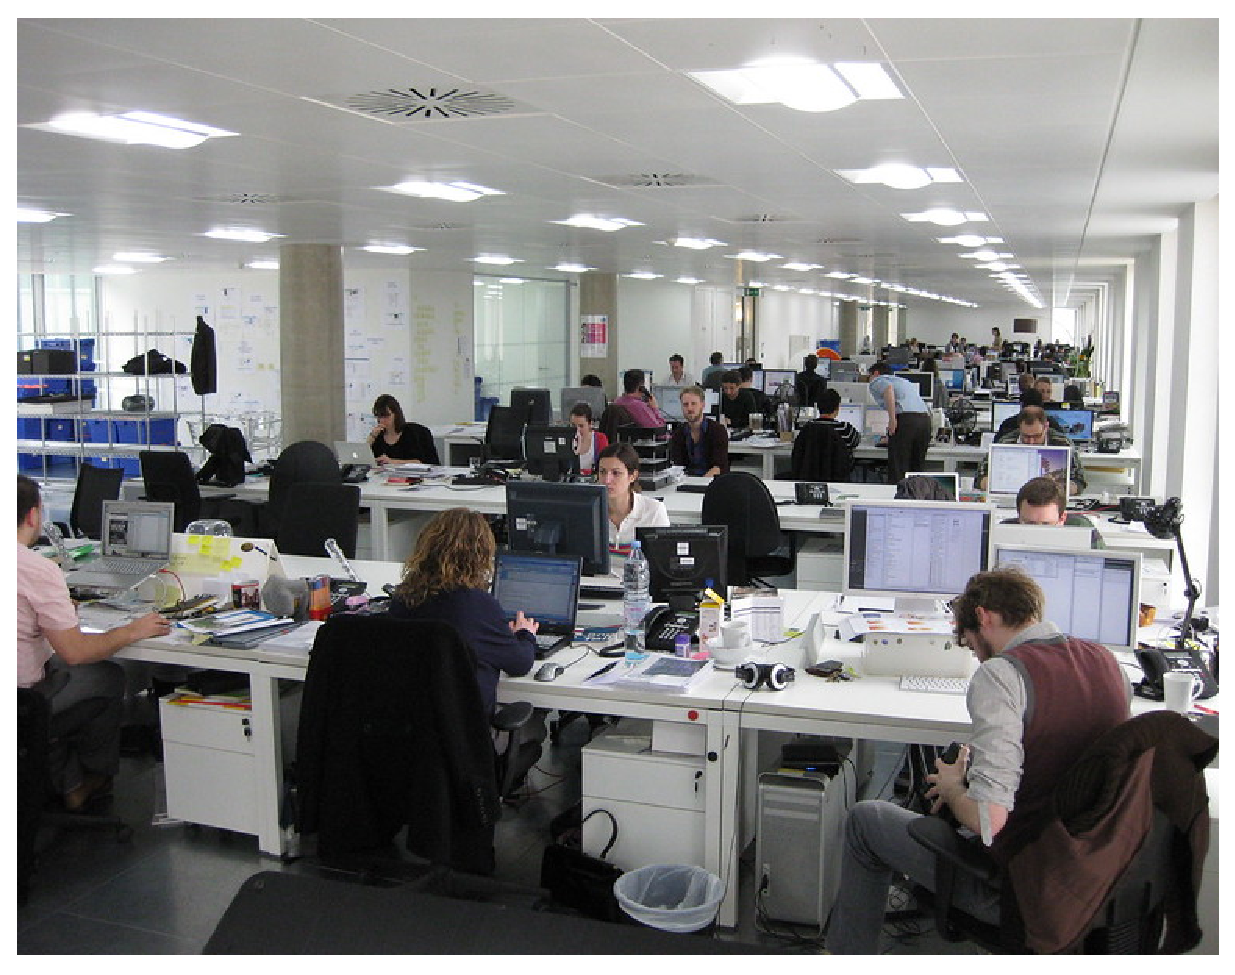
\includegraphics[width=0.73\linewidth,keepaspectratio=true]{images/motivacion01.eps}
	\end{center}
	\begin{flushright}
		\tiny{Photo by: Phil Whitehouse / Flickr}
	\end{flushright}
	%% Author: Phil Whitehouse
	%% https://www.flickr.com/photos/philliecasablanca/3344142642
\end{frame}

\section{Trabajo Eficaz en Equipo}

\subsection{Fundamentos del Trabajo Eficaz en Equipo}

\begin{frame}[c]
	\frametitle{Fundamentos del Trabajo Eficaz en Equipo}
	\begin{block}{Principio Fundamental para el Trabajo Eficaz en Equipo}
		Establecer claramente:
		\begin{itemize}
			\item<2-> El objetivo final que ha de satisfacer el equipo.
			\item<3-> Por qué trabajamos en equipo en lugar de individualmente.
		\end{itemize}
	\end{block}
\end{frame}

\begin{frame}[c]
	\frametitle{Fundamentos del Trabajo Eficaz en Equipo}
	\begin{block}{Regla Fundamental Trabajo Eficaz en Equipo}
		\begin{itemize}[<+->]
			\item Identificar las tareas a realizar.
			\item Tratar de realizar cada tarea de manera autónoma.
			\item Coordinar el progreso de las tareas. 
			\item Tratar de reducir los esfuerzos de coordinación al mismo.
		\end{itemize}
	\end{block}
\end{frame}

\subsection{Pautas para un Eficaz Trabajo en Equipo}

\begin{frame}[c]
	\frametitle{Tipos de Compañeros de Equipo}
	
	\renewcommand{\arraystretch}{2.0}
	
	\begin{center}
		\begin{tabular}{|l|p{2cm}|p{2cm}|p{2cm}|}
			\cline{3-4}
			\multicolumn{2}{l}{}  & \multicolumn{2}{|c|}{Capacidad de  Trabajo} \\ \cline{3-4}
			\multicolumn{2}{l|}{} & \multicolumn{1}{c|}{Alta}                 & 
			\multicolumn{1}{c|}{Baja}         \\ \cline{1-4}
			\multirow{2}{*}{\rotatebox[origin=c]{90}{Afinidad}} & 
			\multicolumn{1}{c|}{Alta} & \multicolumn{1}{c|}{Unicornio} & \multicolumn{1}{c|}{Colega} \\
			\cline{2-4}
			& \multicolumn{1}{c|}{Baja} & \multicolumn{1}{c|}{Compañero}  & \multicolumn{1}{c|}{Huir} \\
			\cline{1-4}
		\end{tabular}
	\end{center}
\end{frame}

\begin{frame}[c]
	\frametitle{Estrategias de Trabajo Eficaz en Equipo}
	\begin{enumerate}[<+->]
		\item Identificar claramente las tareas a realizar.
		\item Hacer las tareas lo más autónomas posibles.
		\item Identificar claramente las dependencias entre tareas.
		\item Asignar con claridad tareas a miembros del equipo.
		\item Evitar trabajadores ociosos.
		\item No existen trabajadores sobrecargados.
		\item No hay trabajadores infrautilizados ni sobrevalorados.
		\item Existen mecanismos de coordinación claramente definidos.
		\item Existen controles y revisiones de calidad.
		\item Hay tiempo para corregir defectos e imperfecciones si se detectasen.
	\end{enumerate}
\end{frame}

\section{Técnicas para el Trabajo Eficaz en Equipo}

\subsection{Celebración de Reuniones}

\begin{frame}[c]
	\frametitle{Celebración de Reuniones}
	\begin{enumerate}[<+->]
		\item Convocar una reunión sólo si es (estrictamente) necesario.
		\item Establecer siempre cuál es el objetivo de la reunión.
		\item Invitar sólo a los participantes imprescindibles. 
		\item Elaborar una miniagenda para la reunión.
		\item Elegir un moderador.
		\item Procurar ser breves y atenerse al objetivo de la reunión.
		\item Elaborar un simple acta para recordar que se acordó en la reunión.
	\end{enumerate}
\end{frame}

\subsection{Toma de Decisiones}

\begin{frame}[c]
	\frametitle{Toma de Decisiones}
	\begin{enumerate}[<+->]
		\item La opinión de todo el mundo merece respeto.
		\item Acotar el tiempo necesario para tomar una decisión.
		\item Adoptar algún sistema de votación.
		\item Adoptar algún mecanismo de desempate.
		\item Una decisión, una vez tomada, está tomada.
		\item Las decisiones son responsabilidad de todo el grupo.
	\end{enumerate}
\end{frame}

\subsection{Controles de Calidad}

\begin{frame}[c]
	\frametitle{Controles de Calidad}
	\begin{enumerate}[<+->]
		\item Todo material producido debe ser verificado por un miembro del grupo distinto al que lo produjo.
		\item Debe verificarse con tiempo suficiente para reaccionar en caso de detectar defectos.
		\item Las tareas de verificación deben estar claramente definidas.
		\item Aplicar la técnica del \emph{abogado del diablo} cuando corresponda.
		\item Si se ve que hay deficiencias en el propio proceso de trabajo en equipo, analizarlas y subsanarlas.
	\end{enumerate}
\end{frame}

\subsection{Herramientas de Trabajo en Grupo}

\begin{frame}[c]
	\frametitle{Herramientas para Trabajo en Equipo}
	\begin{enumerate}[<+->]
		\item Herramientas de Visualización Tareas (e.g., Trello).
		\item Herramientas de Comunicación (e.g., Slack).
		\item Herramientas para Compartir Archivos (e.g., OneDrive).
		\item Herramientas de Versionado (e.g., Git).
		\item Herramientas para Compartir Información (e.g., Sharepoint).
	\end{enumerate}
\end{frame}

\begin{frame}[c]
	\frametitle{Herramientas para Trabajo en Equipo}
	\begin{enumerate}[<+->]
		\item Decidir herramientas de trabajo en equipo a utilizar.
		\item Decidir aplicaciones básicas a utilizar (e.g., Office). 
		\item Asegurarse de que las herramientas son compatibles (UTF-8).
		\item Definir políticas para gestionar los artefactos comunes.
	\end{enumerate}
\end{frame}

\section{Trabajo en Equipo Remoto}

\subsection{Motivación}

\begin{frame}[c]
	\frametitle{¿Por qué tengo que trabajar en la empresa?}
	\begin{center}
		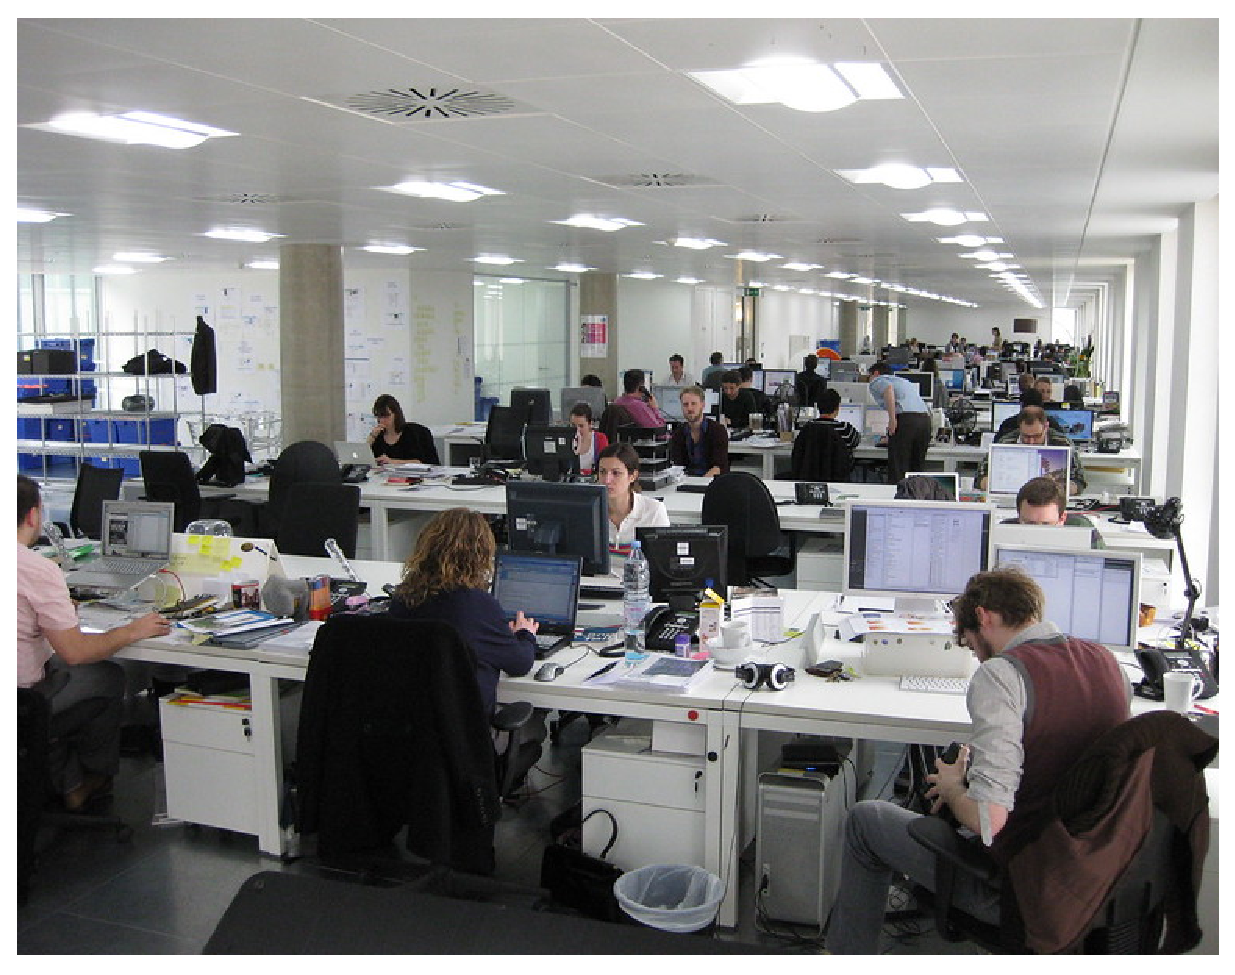
\includegraphics[width=0.75\linewidth,keepaspectratio=true]{images/motivacion01.eps}
	\end{center}
	\begin{flushright}
		\tiny{Photo by: Phil Whitehouse / Flickr}
	\end{flushright}
	%% Author: Phil Whitehouse
	%% https://www.flickr.com/photos/philliecasablanca/3344142642
\end{frame}

\begin{frame}[c]
	\frametitle{Justificaciones para el Trabajo Remoto}
	\begin{enumerate}[<+->]
        \item Conciliación familiar o personal.
        \item Miembros del equipo itinerantes.
        \item Implantación internacional.
        \item Reducción de costes de personal.
	\end{enumerate}
\end{frame}

\subsection{Problemas del Trabajo Remoto}

\begin{frame}[c]
	\frametitle{Problemas del Trabajo Remoto}
	\begin{enumerate}[<+->]
        \item Coordinación de horarios.
        \item Mantener la visión del grupo.
        \item Mantener la calidez de la cercanía.
	\end{enumerate}
\end{frame}

\subsection{Trabajo Remoto Eficaz}

\begin{frame}[c]
	\frametitle{Técnicas para un Trabajo Remoto Eficaz}
	\begin{enumerate}[<+->]
        \item Tener reglas de trabajo claras.
        \item Usar herramientas asíncronas para mantener el contacto.
        \item Tener un mecanismo para hacer claras las decisiones.
        \item Usar videoconferencias para mantener la interacción personal.
        \item Exprimir al máximo las \emph{golden hours}.
        \item En general, no perjudicar al trabajador presencial.
        \item \emph{Todos nosotros} vs \emph{locales y remotos}.
%%        \item \emph{Code reviews} para mantener la consistencia del producto.
	\end{enumerate}
\end{frame}

%\begin{frame}[c]
%	\frametitle{Principios para un Eficaz Trabajo Remoto}
%	\begin{enumerate}[<+->]
%        \item Tener un sitio donde publicar las decisiones globales (y sus justificaciones).
%        \item Políticas de gestión de problemas.
%        \item En general, no perjudicar al trabajador presencial.
%	\end{enumerate}
%\end{frame}

\section{Conclusiones}

\begin{frame}[c]
	\frametitle{Conclusiones}
	\begin{enumerate}[<+->]
		\item Trabajar en equipo no es trabajar todos juntos en el mismo sitio y a la misma hora.
		\item El trabajo en equipo debe ser eficaz. A nadie le gusta perder el tiempo.
		\item El trabajo en equipo debe ser más productivo que el trabajo individual.
	\end{enumerate}
\end{frame}

\end{document}
